\chapter{Future Work}

This chapter lays out some of the potential future directions that BOOM can be taken.  To help facilitate such work, the preliminary design sketches are described below. 

\section{The ROcket Custom Co-processor Interface (ROCC)}

The Rocket in-order processor comes with a ROCC interface that facilitates communication with co-processor/accelerators.  Such accelerators include crypto units (e.g., SHA3) and vector processing units (e.g., the open-source Hwacha vector-thread unit\cite{hwacha}). 

The ROCC interface accepts co-processor commands emitted by {\em committed} instructions run on the ``Control Processor" (e.g., a scalar Rocket core).  Any ROCC commands {\em will} be executed by the co-processor (barring exceptions thrown by the co-processor); nothing speculative can be issued over ROCC. 

Some ROCC instructions will write back data to the Control Processor's scalar register file. 

\subsection{The Demands of the ROCC Interface}


The ROCC interface accepts a ROCC command and up to two register inputs from the Control Processor's scalar register file. 
The ROCC command is actually the entire RISC-V instruction fetched by the Control Processor (a ``ROCC instruction"). Thus, each ROCC queue entry is at least 2*XPRLEN + 32 bits in size (additional ROCC instructions may use the longer instruction formats to encode additional behaviors). \TODO{draw a diagram showing this}

As BOOM does not store the instruction bits in the ROB, a separate data structure (A ``ROCC Reservation Station") will have to hold the instructions until the ROCC instruction can be committed and the ROCC command sent to the co-processor. 

The source operands will also require access to BOOM's register file.  Two possibilities are proposed:

\begin{itemize}
\item ROCC instructions are dispatched to the Issue Window, and scheduled so that they may access the read ports of the register file once the operands are available. The operands are then written into the ROCC Reservation Station, which stores the operands and the instruction bits until they can be sent to the co-processor.  This may require significant state. 
\item ROCC instructions, when they are committed and sent to the ROCC command queue, must somehow access the register file to read out its operands.  If the register file has dynamically scheduled read ports, this may be trivial. Otherwise, some technique to either inject a ROCC micro-op into the issue window or a way to stall the issue window while ROCC accesses the register file will be needed. 
\end{itemize}


\subsection{A Simple One-at-a-Time ROCC Implementation}

The simplest way to add ROCC support to BOOM would be to stall {\em Decode} on every ROCC instruction and wait for the ROB to empty.  Once the ROB is empty, the ROCC instruction can proceed down the BOOM pipeline non-speculatively, and get sent to the ROCC command queue.  BOOM remains stalled until the ROCC accelerator acknowledges the completion of the ROCC instruction and sends back any data to BOOM's register file. Only then can BOOM proceed with its own instructions. 


\subsection{A High-performance ROCC Implementation Using Two-Phase Commit}

While some of the above constraints can be relaxed, the performance of a decoupled co-processor depends on being able to queue up multiple commands while the Control Processor runs ahead (prefetching data and queueing up as many commands as possible).  However, this requirement runs counter to the idea of only sending committed ROCC instructions to the co-processor. 

BOOM's ROB can be augmented to track {\em commit} and {\em non-speculative} pointers. The {\em commit} head pointer tracks the next instruction that BOOM will {\em commit}, i.e., the instruction that will be removed from the ROB and the resources allocated for that instruction will be de-allocated for use by incoming instructions. The {\em non-speculative} head will track which instructions can no longer throw an exception and are no longer speculated under a branch (or other speculative event), i.e., which instructions absolutely will execute and will not throw a pipeline-retry exception. 

This augmentation will allow ROCC instructions to be sent to the ROCC command queue once they are deemed ``non-speculative", but the resources they allocate will not be freed until the ROCC instruction returns an acknowledgement.  This prevents a ROCC instruction that writes a scalar register in BOOM's register file from overwriting a newer instruction's writeback value, a scenario that can occur if the ROCC instruction commits too early, followed by another instruction committing that uses the same ISA register as its writeback destination. 


\subsection{The BOOM Custom Co-processor Interface (BOCC)}

Some accelerators may wish to take advantage of speculative instructions (or even out-of-order issue) to begin executing instructions earlier to maximize de-coupling.  Speculation can be handled by either by epoch tags (if in-order issue is maintained to the co-processor) or by allocating mask bits (to allow for fine-grain killing of instructions). 

\section{The Vector (``V") ISA Extension}

Implementing the Vector Extension in BOOM would open up the ability to leverage performance (or energy-efficiency) improvements in running data-level parallel codes (DLP). 

While it would be relatively easy to add vector arithmetic operations to BOOM, the significant challenges lay in the vector load/store unit. 

\TODO{...}


\section{The Compressed (``C") ISA Extension}

This section describes how to approach adding the Compressed ISA Extension to BOOM.  The Compressed ISA Extension, or RVC  (\url{http://riscv.org/download.html#spec_compressed_isa}) enables smaller, 16 bit encodings of common instructions to decrease the static and dynamic code size.  ``RVC" comes with a number of features that are of particular interest to micro-architects:

\begin{itemize}
\item All 16b instructions map directly into a longer 32b instruction. 
\item 32b instructions have no alignment requirement, and may start on a half-word boundary.
\end{itemize}

\begin{figure}[ht]
	\centering
	\centerline{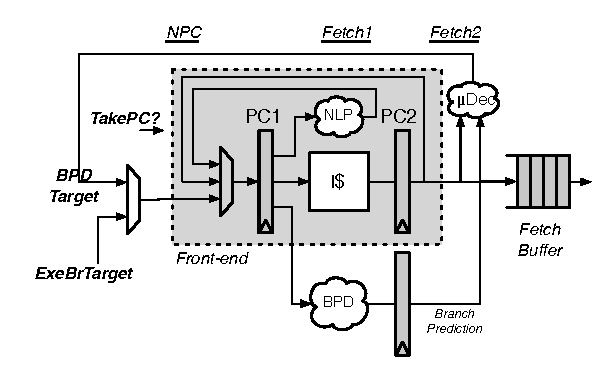
\includegraphics[scale =1] {figures/frontend}}
	\caption{ \small The Fetch Unit. The grey box encompasses the Rocket front-end, which is re-used by BOOM.}
	\label{fig:lsu}
\end{figure}

BOOM re-uses the front-end design from Rocket, a 5-stage in-order core.  BOOM then takes instructions returning (the {\em fetch packet}) from the Rocket front-end, quickly decodes the instructions for branch prediction, and pushes the {\em fetch packet} into the {\em Fetch Buffer}. 


The C Extension provides the following challenges to micro-architects, a few include:

\begin{itemize}
\item Increased decoding complexity (e.g., operands can now move around). 
\item Finding {\em where} the instruction begins. 
\item Tracking down $+4$ assumptions throughout the code base, particularly with branch handling.
\item Unaligned instructions, in particular, running off cache lines and virtual pages. 
\end{itemize}

The last point requires some additional ``statefulness" in the Fetch Unit, as fetching all of the pieces of an instruction may take multiple cycles. 

The following describes the proposed implementation of RVC for BOOM:

\begin{itemize}
\item Implement RVC in the Rocket in-order core.  Done properly, BOOM will then gain RVC support almost entirely for free (modulo any $+4$ assumptions in the code base).
\item Move BOOM's {\em Fetch Buffer} into Rocket's front-end. Rocket will need the statefulness to handle wrap-around issues with fetching unaligned 32 bit instructions.  A non-RVC Rocket core can optionally remove this buffer. 
\item Expand 16-bit instructions as they enter (or possibly exit) the {\em Fetch Buffer}. 
\item Minimize latency by placing 16b$\rightarrow$32b expanders at every half-word start. 
\end{itemize}

\subsection{Challenging Implementation Details}

There are many challenges to implementing RVC in BOOM. First, although all 16 bit encodings map to a 32b version, {\bf the behavior of some 16b instructions are different from their 32b counterparts}!  A JAL instruction writes the address of the following instruction to {\tt rd} - but whether that is $PC+2$ or $PC+4$ depends on whether it's the 16b JAL or a 32b JAL!  Likewise, a mispredicted not-taken branch redirects the fetch unit to $PC+2$ or $PC+4$ depending on whether the branch was the compressed version or not. {\bf Thus, the pipeline must track whether any given instruction was originally a compressed 16b instruction or not.}

The branch prediction units will also require a careful rethink. The BTB tracks which instructions are {\em predicted-taken} branches and redirects the PC as desired. For a superscalar {\em fetch packet}, the BTB must help denote which instruction is to be blamed for the taken prediction to help mask off any invalid instructions that come afterward within the {\em fetch packet}. RVC makes this much more difficult, as some {\em predicted-taken} branches can wrap around fetch groupings/cache lines/virtual page boundaries. Thus, the ``taken" prediction must be attached to a tag-hit on the {\em end} of the branch instruction.  This handles fetching the first part of the branch (and predicting ``not-taken"), then fetching the second part (which hits in the BTB and predicts ``taken"), and only then redirecting the front-end to the predicted-taken PC target. 

One final detail to keep in mind is the i-cache, the instruction translation look-aside buffer (i-TLB), and their interactions with self-modifying RVC code. A RISC-V instruction can legally straddle a virtual page boundary such that the second half is neither in the i-cache nor in the i-TLB. 
